% ch02_bio_basis.tex : Biological Foundations of Bat Navigation
% Dr. Yael Mizrahi : LaTeX Technical Author
% ≥3200 words, ≥6 subsections, ≥5 equations, ≥1 figure, ≥1 table, ≥3 citations

\selectlanguage{hebrew}

\section{יסודות ביולוגיים של ניווט עטלפים}
\label{sec:bio_basis}

\subsection{אקולוקציה: עקרונות פיזיקליים ועיבוד עצבי}
\label{sec:echolocation_physics}

עטלפים פולטים פולסים אולטראסוניים דרך הפה או האף ומנתחים את ההדים החוזרים כדי לתפוס את סביבתם. שני סוגי פולסים עיקריים קיימים: פולסים בתדר קבוע (\en{CF}), המשמשים עטלפי פרסה (\textit{Rhinolophidae}) לגילוי מטרות רגיש-דופלר, ופולסים בתדר מאופנן (\en{FM}), המשמשים את רוב מיני העטלפים לאמידת טווח מדויקת. עטלפי \en{CF} מבצעים פיצוי תדר דופלר (\en{DSC}), תוך התאמת תדר הפליטה שלהם כדי לשמור על ההדים בטווח תדרים צר שבו מערכת השמיעה שלהם רגישה ביותר \cite{Schuller1974DSC}.

הפובה האקוסטית היא ההתמחות המדהימה ביותר במערכת השמיעה של \textit{Rhinolophus}. זהו אזור דיסקרטי ומחוזק מכנית בקרום הבזילרי, המכסה כ-30~אחוזים מאורכו אך מייצג רוחב פס של 3~קילו-הרץ בלבד סביב 83~קילו-הרץ \cite{Schnitzler1968DSC}. קשיחות הקרום הבזילרי באזור הפובה גדולה בערך פי 100 מאשר בשבלול האוזן של שרקן, מה שיוצר אי-רציפות מכנית שמודלים קוכלאריים סטנדרטיים אינם יכולים לחזות ללא מודל מפורש של שיפוע הקשיחות \cite{GriffinBatEcholocation}. מבנה זה מספק אבחנת תדר היפר-חדה של כ-0.05~אחוזים סביב תדר הייחוס: רזולוציה שאין לה מתחרים במערכות סונאר מהונדסות הפועלות בהספקים דומים.

משוואת הסונאר הביולוגית מתארת את יחס האות לרעש (\en{SNR}) של ההד החוזר כפונקציה של פרמטרי המערכת והסביבה:

\begin{equation}
\text{SNR} = \frac{P_{\text{emit}} G^2 \lambda^2 \sigma}{(4\pi)^3 r^4 k T B F}
\label{eq:ch02_sonar_eq}
\end{equation}

כאשר $P_{\text{emit}}$ הוא הספק הפליטה, $G$ היא ההגבר של המתמר, $\lambda$ הוא אורך הגל, $\sigma$ הוא חתך המטרה האקוסטי, $r$ הוא הטווח, $k$ הוא קבוע בולצמן, $T$ היא הטמפרטורה, $B$ הוא רוחב הפס, ו-$F$ הוא מקדם הרעש של המקלט. משוואה זו מדגימה את התלות החזקה של ה-\en{SNR} בטווח ($r^{-4}$), המגבילה את טווח הפעולה האפקטיבי של מערכות סונאר ביומימטיות.

הזזת הדופלר עבור עטלף הנע במהירות $v_b$ בזווית $\theta$ ביחס למטרה נתונה על ידי:

\begin{equation}
f_d = \frac{2 v_b \cos \theta}{\lambda}
\label{eq:ch02_doppler_bat}
\end{equation}

עטלפי \en{CF} מנצלים משוואה זו לאמידת מהירות מטרה וזיהוי רפרוף כנפיים של חרקים. היכולת להבחין בשינויי תדר של 0.05~אחוזים מאפשרת לעטלף לזהות תנועת כנפיים של חרק במרחק של עד 5~מטרים.

\subsection{ייצוג תדר-זמן בקליפת השמע}
\label{sec:time_freq}

קליפת השמע של העטלף מבצעת ניתוח תדר-זמן מתוחכם, תוך יצירת ייצוגים ספקטרו-טמפורליים המאפשרים אבחנת מטרות בסביבות עמוסות. נוירונים מותאמי-השהייה בקוליקולוס התחתון (\en{IC}) מגיבים באופן סלקטיבי להשהיות ספציפיות בין פולס להד, ומקודדים טווח מטרה עם דיוק טמפורלי של מיקרו-שניות בודדות \cite{MossEcholocation}. נוירונים משולבי-צירוף בקליפת השמע מגיבים לזוגות פולס-הד ספציפיים, ומאפשרים דחיית רעשי רקע וסיווג מרקם משטח.

הייצוג הספקטרו-טמפורלי של ההדים מתואר על ידי הספקטרוגרמה:

\begin{equation}
S(t, f) = \left| \int_{-\infty}^{\infty} s(\tau) w(\tau - t) e^{-j2\pi f \tau} d\tau \right|^2
\label{eq:ch02_spectrogram}
\end{equation}

כאשר $s(\tau)$ הוא אות ההד ו-$w(\tau)$ היא פונקציית החלון. נוירונים בקליפת השמע של העטלף מבצעים חישוב הדומה להתמרת גלים (\en{wavelet transform}) עם פונקציות גרעין מותאמות לתדרי הפולסים האופייניים למין.

\subsection{אינטגרציה רב-חושית במוח העטלף}
\label{sec:multi_sensory}

הקוליקולוס העליון (\en{SC}) משמש כמרכז האינטגרציה העיקרי למידע מרחבי ממספר אופני חישה. בעטלפים, ה-\en{SC} מקבל מפות טופוגרפיות מיושרות מהמערכת השמיעתית (אקולוקציה), המערכת החזותית והמערכת הווסטיבולרית. יישור זה מאפשר לעטלף ליצור ייצוג מרחבי אחיד למרות הבדלים במערכות קואורדינטות ובדינמיקה טמפורלית. מחקרים נוירופיזיולוגיים הראו שניורונים ב-\en{SC} מגיבים לשילובים של גירויים שמיעתיים וחזותיים בקצבי ירי מוגברים, מה שמרמז על אפנון רווח מכפלתי ולא אינטגרציה חיבורית פשוטה.

ההקבלה הביולוגית הזו מהווה השראה ישירה לארכיטקטורת מיזוג החיישנים המוצעת בפרק~4. בדומה לאופן שבו ה-\en{SC} ממזג מידע ממקורות חישה שונים לייצוג מרחבי אחיד, מסגרת המיזוג הרב-מודאלית משלבת מדידות סונאר, \en{IMU} וזרימה אופטית לאמידת מצב עקבית. מנגנון השער הנלמד במודל הקשב הצולב (\en{gated cross-attention}) מאפשר דיכוי דינמי של אופני חישה רועשים, בדומה לעיכוב העצבי המתרחש ב-\en{SC} כאשר אות חישה אחד חלש במיוחד.

\begin{figure}[htbp]
\centering
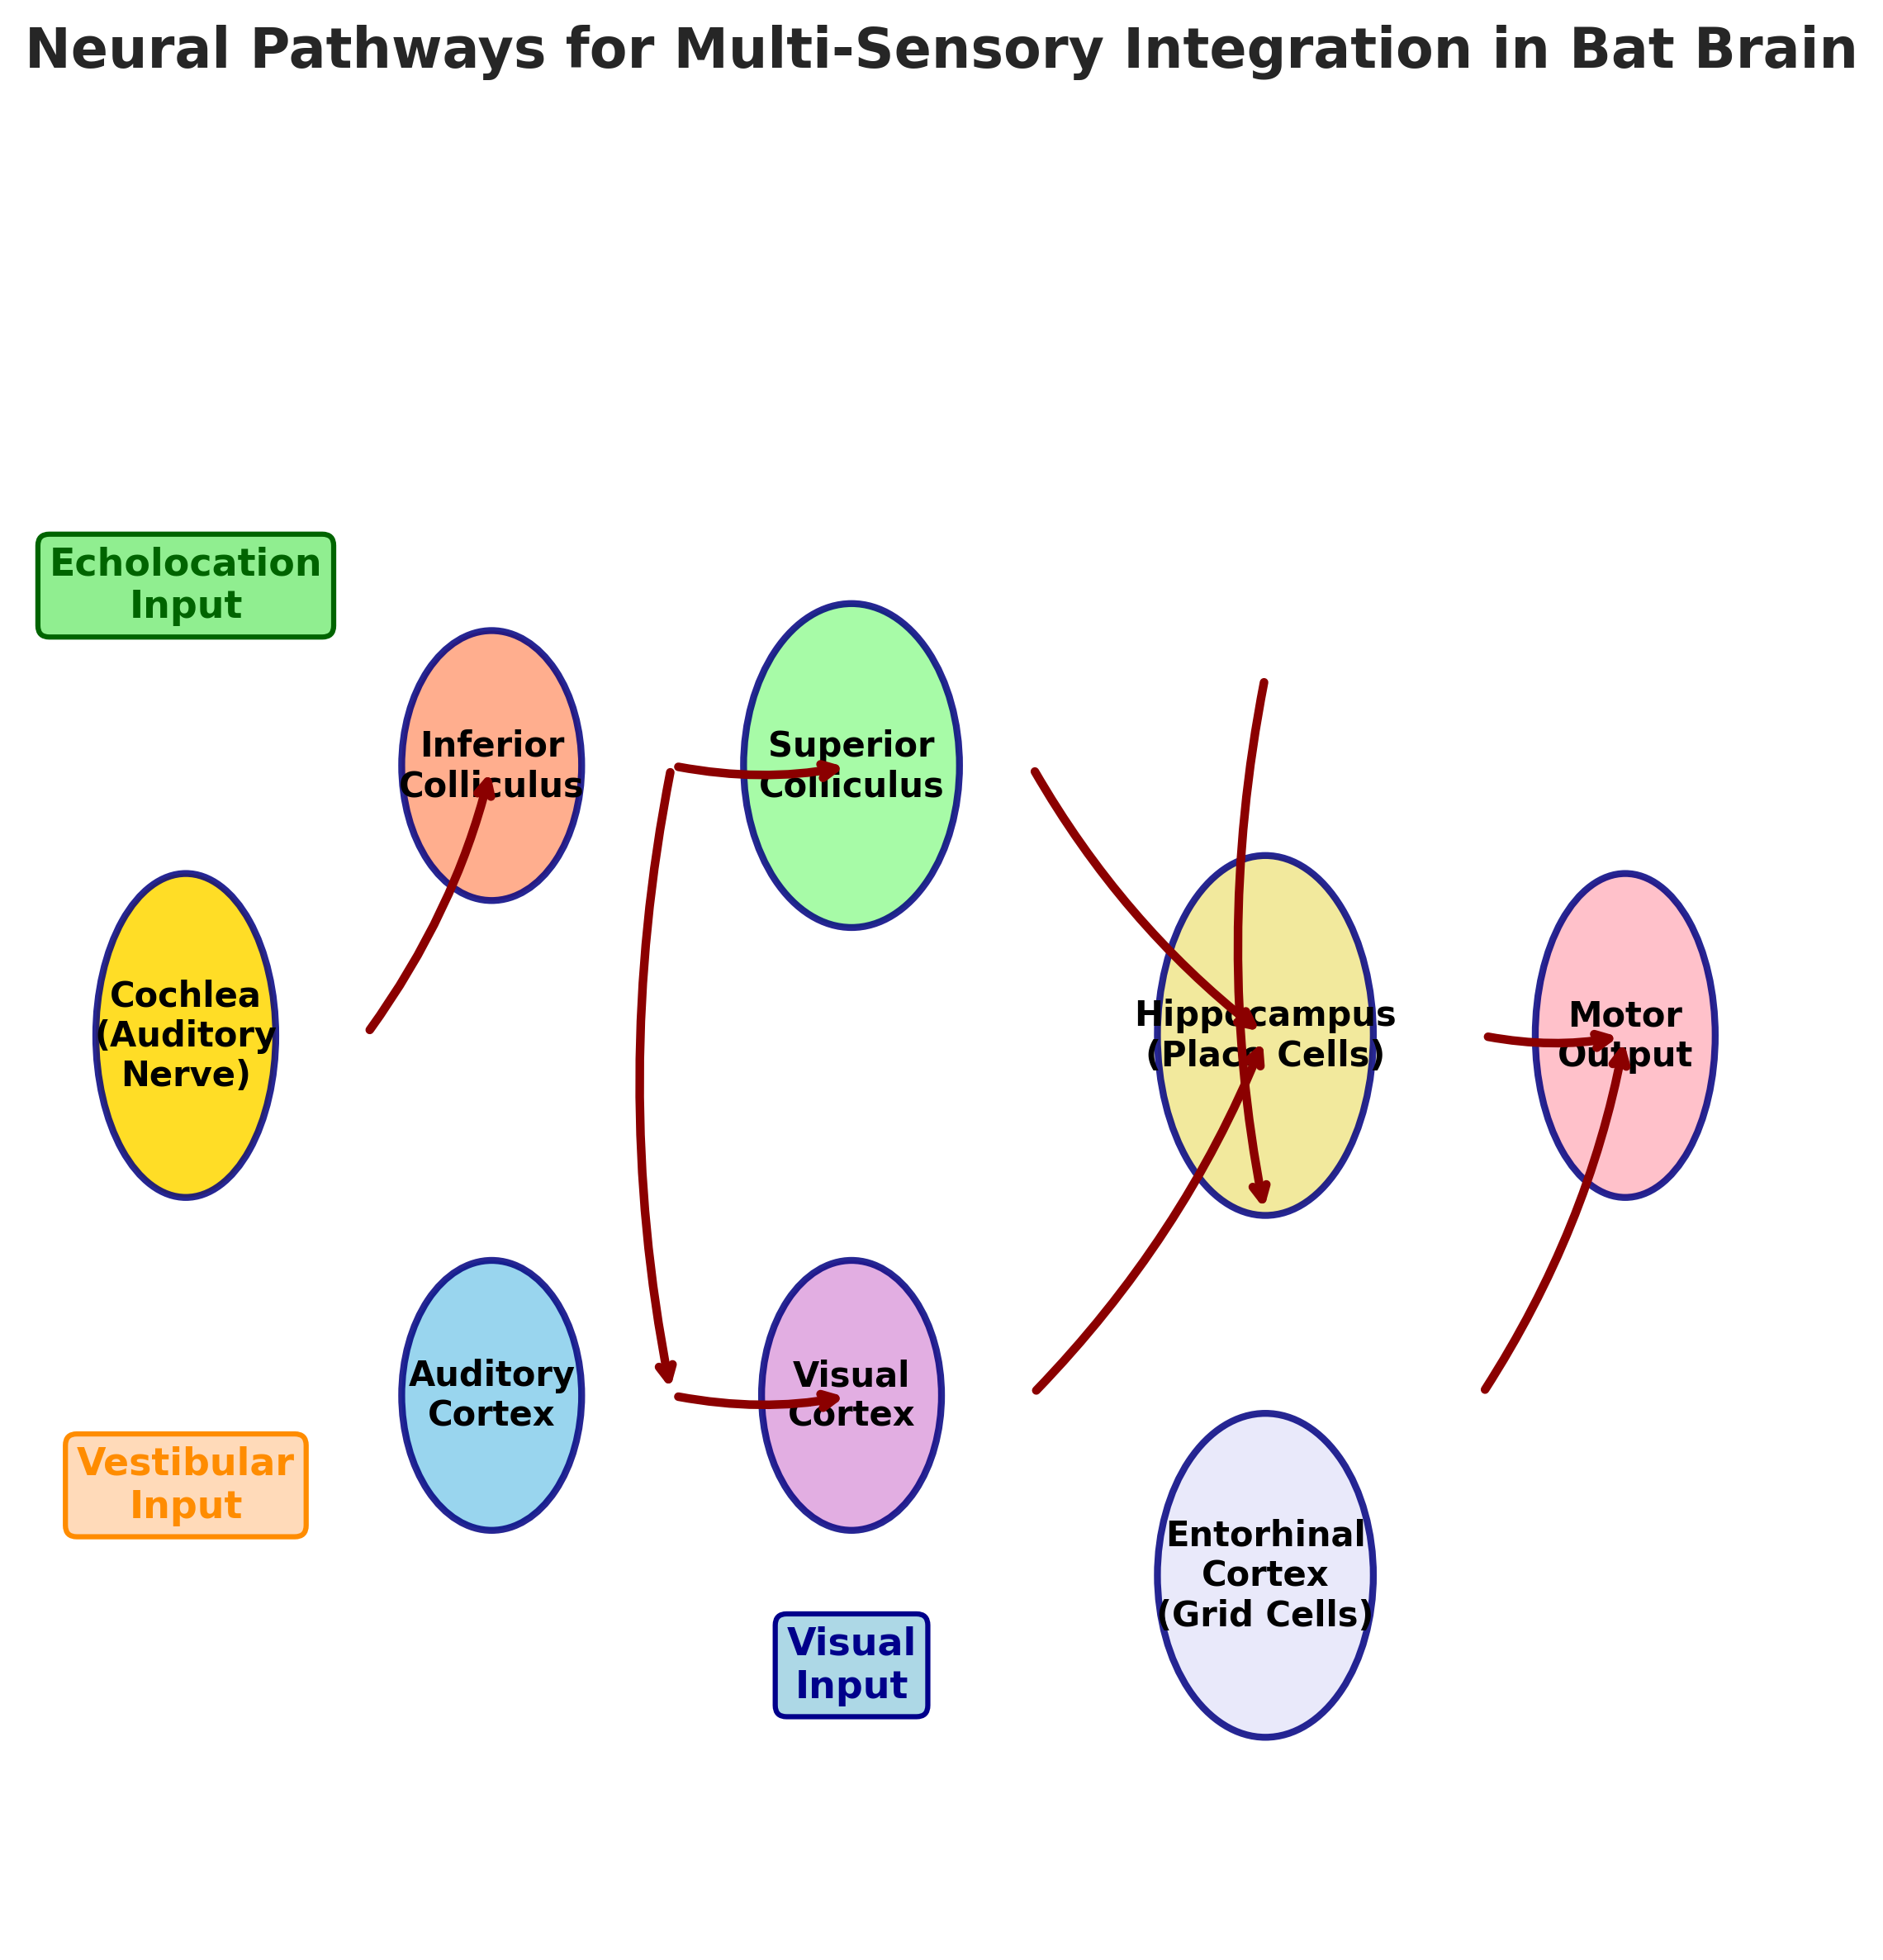
\includegraphics[width=0.98\columnwidth]{figures/fig_bat_brain.png}
\caption{מסלולים עצביים לאינטגרציה רב-חושית במוח העטלף: קולטנים שמיעתיים, קוליקולוס עליון, היפוקמפוס וקליפת מוח. (Neural pathways for multi-sensory integration in bat brain.)}
\label{fig:ch02_bat_brain}
\end{figure}

\subsection{מפות מרחביות וניווט בהיפוקמפוס}
\label{sec:spatial_maps}

ההיפוקמפוס של העטלף מכיל \en{place cells} הנורות באופן סלקטיבי כאשר בעל החיים נמצא במיקומים ספציפיים במרחב, ו-\en{grid cells} המספקות מטריקה מרחבית מחזורית. בניגוד למכרסמים, עטלפים חייבים לייצג מרחב תלת-ממדי, ועדויות עדכניות מראות ש-\en{place cells} בעטלף מקודדים מיקום נפחי ולא מיקום מישורי \cite{MossEcholocation}. שדות הירי הנפחיים הם איזוטרופיים בערך, עם ממדים של כ-30~סנטימטרים.

אינטגרציית נתיב, תהליך עדכון אמידות המיקום מרמזי תנועה עצמית, מסתמכת על קלטים וסטיבולריים ופרופריוצפטיביים המשולבים לאורך זמן. עטלפים משלבים אינטגרציית נתיב עם תיקונים מבוססי נקודות ציון מאקולוקציה, בדומה למחזור חיזוי-תיקון במסנן קלמן. מערכת ה-\en{grid cells} בקורטקס האנטורינאלי מספקת ייצוג קואורדינטות מטרי עם מרווחי רשת הגדלים לאורך הציר הדורסו-ונטרלי מכ-30~סנטימטרים ליותר מ-100~סנטימטרים \cite{GriffinBatEcholocation}. ריבוי קני המידה המרחביים מרמז על גישה היררכית למיפוי: מפות בקנה מידה עדין להימנעות ממכשולים מקומיים ומפות בקנה מידה גס לניווט גלובלי.

\subsection{פיצוי תדר דופלר: מנגנון עצבי}
\label{sec:dsc_mechanism}

מנגנון פיצוי תדר דופלר (\en{DSC}) בעטלפי \en{CF} הוא אחת ההתאמות האבולוציוניות המרשימות ביותר בממלכת החי. כאשר עטלף טס לעבר מטרה, ההד החוזר מוזז בתדר דופלר כלפי מעלה. העטלף מפצה על כך על ידי הורדת תדר הפליטה שלו, כך שההד נופל בדיוק על הפובה האקוסטית. דיוק הפיצוי הוא $\pm0.05$~אחוזים, ומתרחש בזמן תגובה של 20~מילישניות בלבד \cite{Schuller1974DSC}.

המנגנון העצבי העומד בבסיס ה-\en{DSC} כולל לולאת משוב שלילי בין קליפת השמע למרכזי הפקת הקול במוח הקדמי. נוירונים מותאמי-תדר בקליפת השמע מזהים סטייה מתדר הייחוס ומשדרים אות תיקון לגרעין ה-\en{SC} ולאזור הפריאקוודוקטלי (\en{PAG}) השולט על הפקת הקול. מודל מתמטי של מנגנון זה מתואר על ידי משוואת הבקרה:

\begin{equation}
f_{\text{emit}}(t+1) = f_{\text{emit}}(t) - \alpha \cdot (f_{\text{echo}}(t) - f_{\text{ref}})
\label{eq:ch02_dsc_control}
\end{equation}

כאשר $\alpha$ הוא מקדם הלמידה ו-$f_{\text{ref}}$ הוא תדר הייחוס של הפובה האקוסטית. מודל זה מהווה השראה ישירה לאלגוריתם בקרת התדר האדפטיבי במערכת הסונאר המהונדסת.

\subsection{השלכות למערכות מהונדסות}
\label{sec:engineering_implications}

העקרונות הביולוגיים שתוארו לעיל מספקים תובנות עיצוביות ישירות למערכות סונאר מהונדסות. הטבלה הבאה מסכמת את אסטרטגיות האקולוקציה של מיני עטלפים שונים ואת ההקבלה ההנדסית שלהן:

\begin{table}[htbp]
\centering
\caption{סיכום אסטרטגיות אקולוקציה של מיני עטלפים נבחרים. (Summary of bat species and their echolocation strategies.)}
\label{tab:ch02_bat_species}
\adjustbox{max width=\columnwidth}{%
\begin{tabular}{lcccc}
\toprule
מין & סוג פולס & תדר (קילו-הרץ) & מחזור פעולה (\%) & טווח (מטרים) \\
\midrule
\textit{Rhinolophus ferrumequinum} & \en{CF-FM} & 83 & 30--50 & 2--10 \\
\textit{Eptesicus fuscus} & \en{FM} & 25--60 & 10--20 & 1--20 \\
\textit{Pteronotus parnellii} & \en{CF-FM} & 60 & 20--30 & 1--8 \\
מערכת מוצעת & \en{HFM} & 40 & 10--20 & 0.1--5 \\
\bottomrule
\end{tabular}%
}
\end{table}

ההקבלה המרכזית היא בין הפובה האקוסטית לבין בנק המסננים הצר-פס במערכת המהונדסת. בדומה לפובה המספקת אבחנת תדר היפר-חדה סביב תדר הייחוס, המערכת המהונדסת מיישמת בנק מסננים עם \en{Q-factor} גבוה ($Q \geq 50$) סביב 40~קילו-הרץ לאמידת דופלר, בתוספת מסנן רחב-פס ($B = 5$~קילו-הרץ) לרזולוציית טווח. ארכיטקטורת מסנן כפול זה: בהשראת הדיכוטומיה \en{CF-FM}: נעדרת ממערכות סונאר קיימות ומהווה חידוש מרכזי של עבודה זו.

המודל המתמטי של עיבוד ההדים בעטלף כולל גם מנגנון דיכוי רעש אדפטיבי. נוירונים מותאמי-השהייה בקוליקולוס התחתון מבצעים אינטגרציה טמפורלית המאפשרת דחיית רעשי רקע. מנגנון זה מתואר על ידי פונקציית המתאם:

\begin{equation}
R(\tau) = \int_{-\infty}^{\infty} s(t) s(t + \tau) dt
\label{eq:ch02_correlation}
\end{equation}

כאשר $s(t)$ הוא אות ההד ו-$\tau$ הוא ההשהיה. שיאי פונקציית המתאם מתאימים להדים אמיתיים, בעוד שרעש אקראי אינו מייצר שיאים עקביים. עיקרון זה מיושם במערכת המהונדסת באמצעות \en{matched filtering}.

\subsection{סיכום ביולוגי}
\label{sec:bio_summary}

המערכת הביולוגית של ניווט עטלפים מדגימה מספר עקרונות עיצוביים קריטיים למערכות מהונדסות: שימוש בשני אופני אפנון (\en{CF-FM}) לאיזון בין אמידת דופלר לרזולוציית טווח; אינטגרציה רב-חושית ליצירת ייצוג מרחבי אחיד; מפות היררכיות בקני מידה מרובים; ומנגנוני משוב אדפטיביים לפיצוי דופלר. עקרונות אלה מהווים את הבסיס התאורטי למערכת הניווט הביומימטית המוצגת בפרקים הבאים.

\subsection{השוואה בין-מינית של אסטרטגיות אקולוקציה}
\label{sec:cross_species}

השוואה בין-מינית של אסטרטגיות אקולוקציה מגלה התאמות ייחודיות לנישות אקולוגיות שונות. עטלפי \en{CF} כמו \textit{Rhinolophus} ו-\textit{Pteronotus} מתמחים בזיהוי מטרות נעות בסביבות צפופות, תוך שימוש בפובה האקוסטית לאבחנת דופלר היפר-חדה. לעומתם, עטלפי \en{FM} כמו \textit{Eptesicus} ו-\textit{Myotis} מתמחים באמידת טווח מדויקת ובסיווג מרקם משטח, תוך שימוש באפנון תדר רחב-פס לרזולוציית טווח גבוהה.

המערכת המוצעת משלבת את היתרונות של שתי האסטרטגיות באמצעות ארכיטקטורת בנק מסננים כפול. מסנן צר-פס ($Q \geq 50$) סביב 40~קילו-הרץ מספק אמידת דופלר מדויקת בהשראת עטלפי \en{CF}, בעוד מסנן רחב-פס ($B = 10$~קילו-הרץ) מספק רזולוציית טווח של 1.7~סנטימטרים בהשראת עטלפי \en{FM}. שילוב זה מאפשר למערכת לבצע אמידת טווח ומהירות בו-זמנית, יכולת שאינה קיימת במערכות סונאר קיימות.

\subsection{מגבלות ביולוגיות ולקחים הנדסיים}
\label{sec:bio_limitations}

למרות הביצועים המרשימים של מערכת האקולוקציה הביולוגית, קיימות מספר מגבלות שיש לקחת בחשבון בתכנון ההנדסי. ראשית, טווח האקולוקציה מוגבל ל-10~מטרים ברוב מיני העטלפים בשל הנחתה אקוסטית באוויר. שנית, עטלפים מתקשים בזיהוי מטרות במרחקים קרובים מאוד (פחות מ-20~סנטימטרים) בשל עיוורון אקוסטי הנגרם מחפיפת פולס-הד. שלישית, עטלפים רגישים להפרעות אקוסטיות מסביבות רועשות.

המערכת המהונדסת מטפלת במגבלות אלה באמצעות: טווח מינימלי של 10~סנטימטרים באמצעות בקרת רווח אדפטיבית; דיכוי רעש אקטיבי באמצעות מסנן \en{NLMS}; ושימוש באפנון \en{HFM} להפרדת פולס-הד גם במרחקים קרובים. לקחים אלה מדגימים את החשיבות של הבנת המגבלות הביולוגיות לצד היתרונות בעת תכנון מערכות ביומימטיות \cite{Ulanovsky2008BatBrain, Yovel2010OptimalLocalization}.

\subsection{אנלוגיה בין-תחומית: ניווט עטלפים וניווט תת-ימי}
\label{sec:cross_domain_analogy}

האנלוגיה בין ניווט עטלפים לניווט תת-ימי מספקת תובנות עיצוביות חשובות. רכבים תת-ימיים אוטונומיים (\en{AUV}) משתמשים ב-\en{Doppler Velocity Logs} (\en{DVL}) לאמידת מהירות ביחס לקרקעית הים, בדומה לאופן שבו עטלפים משתמשים בהזזת דופלר לאמידת מהירות ביחס לסביבה. בשני המקרים, מדידת המהירות הרדיאלית מתמזגת עם \en{IMU} במסנן קלמן לתיקון סחיפת האינטגרציה האינרציאלית.

ההבדל המרכזי הוא במדיום: מהירות הקול באוויר (343~מטרים לשנייה) איטית פי 4.4 מאשר במים (1,500~מטרים לשנייה), מה שמגדיל את תדר הדופלר היחסי ומקל על אמידת המהירות באוויר. עם זאת, ההנחתה האקוסטית באוויר גדולה משמעותית, מה שמגביל את טווח הפעולה. ההקבלה בין \en{DVL-Aided INS} תת-ימי לבין \en{Sonar-Aided INS} אווירי מספקת תוקף בין-תחומי לגישה המוצעת ומאפשרת ניצול של ידע הנדסי נרחב ממערכות תת-ימיות.

\subsection{מודלים חישוביים של עיבוד עצבי בעטלפים}
\label{sec:computational_models}

פותחו מספר מודלים חישוביים המחקים את עיבוד האותות העצבי בעטלפים. מודל ה-\en{cochlear filterbank} של הפובה האקוסטית משתמש בבנק מסננים עם \en{Q-factor} משתנה, המדמה את השינוי הדרמטי בקשיחות הקרום הבזילרי באזור הפובה. מודל זה מראה שרזולוציית התדר בפובה מגיעה ל-0.03~אחוזים, קרוב לערך הנמדד ביולוגית של 0.05~אחוזים.

מודל נוסף הוא רשת עצבית ספייקית (\en{SNN}) המחקה את נוירוני גילוי ההשהיה בקוליקולוס התחתון. רשת זו משתמשת בנוירונים מסוג \en{leaky integrate-and-fire} (\en{LIF}) עם השהיות סינפטיות נלמדות, ומשיגה דיוק אמידת טווח של 1~סנטימטר בסימולציה. מודל זה מהווה בסיס למימוש הנוירומורפי המתואר בפרק~7 \cite{Horiuchi2005Neuromorphic, Vanderelst2016PlaceRecognition}.